%!TEX root = main.tex
\vspace{-10pt}
\section{Perspective Resolution\label{perspective}}
% \subsection{Worker Clustering}
As discussed in Section~\ref{sec:error}, worker disagreements often arise in crowdsourced segmentation due to differing worker perspectives on large tile regions. To resolve this issue, we develop a clustering-based preprocessing approach.
% is based on the intuition that workers with similar perspectives  will have segmentations that are closer to each other. 
We capture the similarity between a pair of workers by computing the Jaccard score between their segmentations and perform spectral clustering to separate workers into clusters. Figure \ref{error_examples} bottom illustrates how spectral clustering is capable of dividing the worker responses into clusters with meaningful semantic associations, reflecting the crowd's diversity of perspectives in completing same task. Clustering results can be used as a preprocessing step to any of the quality evaluation algorithms by keeping only the segmentations that belong to the largest cluster, which is typically free of any semantic errors.
    % \begin{figure}[h!]
    %   \centering
    %   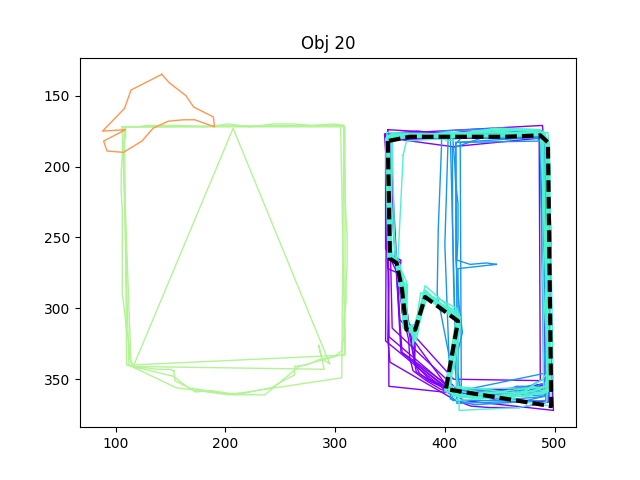
\includegraphics[width=\textwidth]{plots/20.png}
    %   \caption{Example image showing clustering performed on the same object from Figure \ref{error_examples}.}
    %   \label{cluster_example}
    % \end{figure}
\par In addition, clustering offers an additional benefit of preserving worker's semantic intentions in the case where there are multiple instances of different errors. For example, while the green cluster in in Figure~\ref{error_examples} bottom right are considered \textit{bad} annotations for the particular task (`computer'), this cluster of annotation can provide more data for another semantic segmentation task ``monitor''. A potential future work includes adding additional crowdsourcing tasks for semantic labeling of clusters (which is cheaper and more accurate than segmentation) to enable reuse of annotations across multiple objects and lower the cost of data collection. 